\documentclass[aspectratio=169,11pt]{beamer}
\usetheme{AnnArbor}
\usecolortheme{seahorse}
\usepackage{fontspec}
\setmainfont{Noto Sans}
\setsansfont{Noto Sans}
\setmonofont{DejaVu Sans Mono}[Scale=0.85]
\usepackage{booktabs,tabularx,array,amsmath,amssymb}
\usepackage{tikz}
\usetikzlibrary{arrows.meta,positioning,calc}
\usepackage{listings}
\usepackage{xcolor}
\usepackage{hyperref}
\definecolor{BlueMain}{HTML}{17365D}
\definecolor{TealMain}{HTML}{007F79}
\definecolor{OrangeMain}{HTML}{B86C13}
\definecolor{CodeBg}{HTML}{F4F7FB}
\definecolor{CodeText}{HTML}{26344C}
\setbeamercolor{structure}{fg=BlueMain}
\setbeamercolor{frametitle}{fg=white,bg=BlueMain}
\setbeamercolor{title}{fg=white,bg=BlueMain}
\setbeamercolor{palette primary}{fg=white,bg=BlueMain}
\setbeamercolor{palette secondary}{fg=white,bg=TealMain}
\setbeamercolor{palette tertiary}{fg=white,bg=BlueMain}
\setbeamercolor{block title}{fg=white,bg=BlueMain}
\setbeamercolor{block body}{fg=black,bg=BlueMain!6}
\setbeamercolor{block title alerted}{fg=white,bg=OrangeMain}
\setbeamercolor{block body alerted}{fg=black,bg=OrangeMain!8}
\setbeamercolor{block title example}{fg=white,bg=TealMain}
\setbeamercolor{block body example}{fg=black,bg=TealMain!7}
\setbeamercolor{insight}{fg=BlueMain,bg=BlueMain!7}
\setbeamersize{text margin left=8mm,text margin right=8mm}
\setbeamertemplate{navigation symbols}{}
\setbeamertemplate{headline}{}
\setbeamerfont{frametitle}{size=\large,series=\bfseries}
\setbeamerfont{normal text}{size=\small}
\setbeamertemplate{footline}{%
  \leavevmode\hbox{%
   \begin{beamercolorbox}[wd=.79\paperwidth,ht=2.6ex,dp=1.1ex,leftskip=2ex]{palette primary}%
   \scriptsize DBMS · MySQL Window Functions
   \end{beamercolorbox}%
   \begin{beamercolorbox}[wd=.21\paperwidth,ht=2.6ex,dp=1.1ex,rightskip=2ex plus1fil]{palette secondary}%
   \scriptsize\hfill\insertframenumber/\inserttotalframenumber
   \end{beamercolorbox}%
  }
}
\newcommand{\code}[1]{{\small\ttfamily\detokenize{#1}}}
\lstset{
  language=SQL,
  basicstyle=\ttfamily\fontsize{8.5}{9.8}\selectfont,
  keywordstyle=\color{BlueMain}\bfseries,
  commentstyle=\color{TealMain!80!black}\itshape,
  stringstyle=\color{OrangeMain!90!black},
  identifierstyle=\color{CodeText},
  backgroundcolor=\color{CodeBg},
  frame=single,rulecolor=\color{BlueMain!12},
  frameround=tttt,
  breaklines=true,breakatwhitespace=false,
  showstringspaces=false,
  columns=fullflexible,
  xleftmargin=3pt,xrightmargin=3pt,
  aboveskip=5pt,belowskip=6pt,
  tabsize=2,
  morekeywords={OVER,PARTITION,ROWS,RANGE,PRECEDING,FOLLOWING,UNBOUNDED,CURRENT,WINDOW,ROW_NUMBER,DENSE_RANK,RANK,NTILE,PERCENT_RANK,CUME_DIST,FIRST_VALUE,LAST_VALUE,NTH_VALUE,LAG,LEAD,WITH,DATE_FORMAT,DATEDIFF},
}
\hypersetup{colorlinks=true,urlcolor=TealMain}
\title{MySQL Window Functions}
\subtitle{Phân tích dữ liệu bằng SQL}
\author{DBMS Course}
\date{2026}
\begin{document}

% ---- Slide 1 ----
\begin{frame}[fragile]{MySQL Window Functions}

\vspace{1.0em}
\begin{center}
{\Large\bfseries Phân tích dữ liệu bằng SQL}\par
\vspace{0.6em}
{\normalsize Cửa sổ phân tích · Xếp hạng · Tổng lũy kế · So sánh chuỗi thời gian}\par
\vspace{1.7em}

\begin{tikzpicture}[node distance=0.15cm]
\node[draw=BlueMain,thick,rounded corners=6pt,fill=BlueMain!6,minimum width=3cm,minimum height=1.0cm] (a) {\textbf{PARTITION BY}};
\node[draw=TealMain,thick,rounded corners=6pt,fill=TealMain!7,minimum width=2.6cm,minimum height=1.0cm,right=of a] (b) {\textbf{ORDER BY}};
\node[draw=OrangeMain,thick,rounded corners=6pt,fill=OrangeMain!8,minimum width=2.5cm,minimum height=1.0cm,right=of b] (c) {\textbf{FRAME}};
\draw[-{Stealth[length=2mm]},very thick,gray] (a) -- (b);
\draw[-{Stealth[length=2mm]},very thick,gray] (b) -- (c);
\end{tikzpicture}\par
\vspace{1.3em}
{\small Môi trường: MySQL 8.0+ · Schema: \code{window_function_lab}}
\end{center}

\end{frame}

% ---- Slide 2 ----
\begin{frame}[fragile]{Mục tiêu học tập}
\begin{itemize}
\item Hiểu sự khác nhau giữa \code{GROUP BY} và \code{OVER(...)}.
\item Viết được \code{PARTITION BY}, \code{ORDER BY} và frame.
\item Tính tổng theo nhóm, tỷ trọng, running total, moving average.
\item Xếp hạng và giải bài toán top-\(N\) theo nhóm.
\item So sánh các dòng liên tiếp bằng \code{LAG/LEAD}; lấy giá trị đầu/cuối.
\item Sử dụng \code{NTILE}, \code{PERCENT_RANK}, \code{CUME_DIST}.
\item Kết hợp CTE, named windows và nhận diện lỗi truy vấn thường gặp.
\end{itemize}
\end{frame}

% ---- Slide 3 ----
\begin{frame}[fragile]{Lộ trình bài giảng}

\begin{enumerate}
\setlength{\itemsep}{0.55em}
\item \textbf{Nền tảng:} Dữ liệu, GROUP BY, cú pháp OVER.
\item \textbf{Aggregate windows:} Tỷ trọng, running total, moving average.
\item \textbf{Ranking:} ROW\_NUMBER, RANK, DENSE\_RANK, top-N.
\item \textbf{Value và distribution:} LAG, LEAD, FIRST/LAST/NTH, NTILE.
\item \textbf{Nâng cao:} ROWS/RANGE, WINDOW clause, aggregate rồi window.
\item \textbf{Thực hành:} Constraints, performance, bài tập tổng hợp.
\end{enumerate}

\end{frame}

% ---- Slide 4 ----
\begin{frame}[fragile]{Dataset: bảng sales}
\begin{columns}[T,onlytextwidth]
\column{0.64\textwidth}
\begin{lstlisting}[basicstyle=\ttfamily\fontsize{7.6}{8.799999999999999}\selectfont]
CREATE TABLE sales (
  sale_id BIGINT UNSIGNED AUTO_INCREMENT PRIMARY KEY,
  sales_rep VARCHAR(50) NOT NULL,
  region VARCHAR(30) NOT NULL,
  product_name VARCHAR(100) NOT NULL,
  sale_date DATE NOT NULL,
  amount DECIMAL(12,2) NOT NULL,
  CHECK (amount > 0),
  INDEX idx_rep_date (sales_rep, sale_date, sale_id),
  INDEX idx_region_amount (region, amount)
);
\end{lstlisting}
\column{0.36\textwidth}

\textbf{Cấu trúc dữ liệu}\par
\vspace{0.3em}
\begin{itemize}
\item 1 row = 1 giao dịch bán hàng.
\item Hai khu vực: \textbf{North}, \textbf{South}.
\item Bốn nhân viên: \textbf{An, Binh, Chau, Dung}.
\item 21 dòng, có doanh thu bằng nhau và giao dịch cùng ngày.
\end{itemize}

\end{columns}
\end{frame}

% ---- Slide 5 ----
\begin{frame}[fragile]{Dataset: các thống kê kiểm tra}

\begin{columns}[T,onlytextwidth]
\column{.52\textwidth}
\textbf{Tổng doanh thu từng vùng}
\begin{center}
\renewcommand{\arraystretch}{1.18}
\begin{tabular}{lrr}
\toprule
Region & Rows & Revenue \\
\midrule
North & 11 & 7,350.00 \\
South & 10 & 6,850.00 \\
\textbf{All} & \textbf{21} & \textbf{14,200.00} \\
\bottomrule
\end{tabular}
\end{center}
\column{.48\textwidth}
\textbf{Tổng theo nhân viên}
\begin{center}
\renewcommand{\arraystretch}{1.18}
\begin{tabular}{lr}
\toprule
Sales rep & Revenue \\
\midrule
An & 4,200.00 \\
Binh & 3,150.00 \\
Chau & 3,400.00 \\
Dung & 3,450.00 \\
\bottomrule
\end{tabular}
\end{center}
\end{columns}
\begin{beamercolorbox}[wd=\linewidth,sep=1.1ex,rounded=true]{insight}
\textbf{Chú ý:} Những con số minh họa trong slide được tính từ chính 21 giao dịch mẫu. Script tạo dữ liệu đi kèm tài liệu.
\end{beamercolorbox}
\end{frame}

% ---- Slide 6 ----
\begin{frame}[fragile]{GROUP BY và Window Function}

\begin{center}
\begin{tikzpicture}[node distance=0.65cm, every node/.style={font=\small}]
\node[draw,rounded corners,fill=BlueMain!8,minimum width=3cm,minimum height=1.1cm] (d) {21 rows giao dịch};
\node[draw,rounded corners,fill=OrangeMain!13,minimum width=3.25cm,minimum height=.85cm,right=1.0cm of d,yshift=.9cm] (g) {GROUP BY region};
\node[draw,rounded corners,fill=TealMain!10,minimum width=3.25cm,minimum height=.85cm,right=1.0cm of d,yshift=-.9cm] (w) {SUM(...) OVER(...)};
\node[draw,rounded corners,fill=OrangeMain!5,minimum width=2.5cm,minimum height=.85cm,right=.75cm of g] (gr) {2 rows kết quả};
\node[draw,rounded corners,fill=TealMain!5,minimum width=2.5cm,minimum height=.85cm,right=.75cm of w] (wr) {21 rows kết quả};
\draw[-{Stealth},thick] (d.east) -- (g.west); \draw[-{Stealth},thick] (d.east) -- (w.west);
\draw[-{Stealth},thick] (g.east) -- (gr.west); \draw[-{Stealth},thick] (w.east) -- (wr.west);
\end{tikzpicture}
\end{center}
\vspace{1.1em}
\begin{center}
\renewcommand{\arraystretch}{1.18}
\begin{tabular}{lll}
\toprule
 & GROUP BY & Window function \\
\midrule
Đơn vị đầu ra & Mỗi nhóm & Mỗi dòng chi tiết \\
Kết quả & Tổng hợp & Phân tích gắn vào từng dòng \\
Phù hợp & Báo cáo tóm tắt & Bảng giao dịch + KPI \\
\bottomrule
\end{tabular}
\end{center}
\end{frame}

% ---- Slide 7 ----
\begin{frame}[fragile]{Ví dụ GROUP BY: chỉ lấy kết quả tổng hợp}
\begin{columns}[T,onlytextwidth]
\column{0.55\textwidth}
\begin{lstlisting}[basicstyle=\ttfamily\fontsize{9}{10.2}\selectfont]
SELECT region,
       SUM(amount) AS revenue
FROM sales
GROUP BY region;
\end{lstlisting}
\column{0.45\textwidth}

\textbf{Output}
\begin{center}
\renewcommand{\arraystretch}{1.18}
\begin{tabular}{lr}
\toprule
region & revenue \\
\midrule
North & 7,350.00 \\
South & 6,850.00 \\
\bottomrule
\end{tabular}
\end{center}\small\textit{21 giao dịch được gom còn 2 rows.}
\end{columns}
\end{frame}

% ---- Slide 8 ----
\begin{frame}[fragile]{Ví dụ Window SUM: giữ dữ liệu giao dịch}
\begin{columns}[T,onlytextwidth]
\column{0.59\textwidth}
\begin{lstlisting}[basicstyle=\ttfamily\fontsize{8.3}{9.5}\selectfont]
SELECT sale_id,
       region,
       amount,
       SUM(amount) OVER (
         PARTITION BY region
       ) AS region_total
FROM sales
ORDER BY region, sale_id;
\end{lstlisting}
\column{0.41\textwidth}

\footnotesize\textbf{Output rút gọn}
\begin{center}
\renewcommand{\arraystretch}{1.18}
\begin{tabular}{rlrr}
\toprule
sale & region & amount & total \\
\midrule
1 & North & 1,200 & 7,350 \\
2 & North & 200 & 7,350 \\
12 & South & 1,500 & 6,850 \\
13 & South & 200 & 6,850 \\
\bottomrule
\end{tabular}
\end{center}\small\textit{Giữ 21 rows, thêm tổng của region tương ứng.}
\end{columns}
\end{frame}

% ---- Slide 9 ----
\begin{frame}[fragile]{Cú pháp của OVER()}

\begin{lstlisting}[basicstyle=\ttfamily\fontsize{10}{11.2}\selectfont]
function_name(expression) OVER (
  [PARTITION BY expression [, ...]]
  [ORDER BY expression [ASC | DESC] [, ...]]
  [ROWS | RANGE frame_specification]
)
\end{lstlisting}
\vspace{0.9em}
\begin{center}
\renewcommand{\arraystretch}{1.18}
\begin{tabular}{ll}
\toprule
Thành phần & Câu hỏi \\
\midrule
\code{PARTITION BY} & Chia nhóm để tính riêng? \\
\code{ORDER BY} & Thứ tự logic trong từng nhóm? \\
\code{Frame} & Tại dòng hiện tại sẽ xét những rows nào? \\
\bottomrule
\end{tabular}
\end{center}\begin{beamercolorbox}[wd=\linewidth,sep=1.1ex,rounded=true]{insight}
Không viết \code{PARTITION BY} $\Rightarrow$ toàn bộ input của query block thuộc một partition.
\end{beamercolorbox}
\end{frame}

% ---- Slide 10 ----
\begin{frame}[fragile]{OVER() rỗng và PARTITION BY}
\begin{columns}[T,onlytextwidth]
\column{0.57\textwidth}
\begin{lstlisting}[basicstyle=\ttfamily\fontsize{8.3}{9.5}\selectfont]
SELECT sale_id, region, amount,
       SUM(amount) OVER ()
         AS company_total,
       SUM(amount) OVER (
         PARTITION BY region
       ) AS region_total
FROM sales;
\end{lstlisting}
\column{0.43\textwidth}

\textbf{Cách đọc}\par
\vspace{.6em}
\begin{itemize}
\item \code{OVER()}: tổng \textbf{14,200} tại mọi row.
\item \code{PARTITION BY region}: North = \textbf{7,350}; South = \textbf{6,850}.
\item Không làm thay đổi số lượng giao dịch đầu ra.
\end{itemize}

\end{columns}
\end{frame}

% ---- Slide 11 ----
\begin{frame}[fragile]{Hai loại ORDER BY rất khác nhau}
\begin{columns}[T,onlytextwidth]
\column{0.62\textwidth}
\begin{lstlisting}[basicstyle=\ttfamily\fontsize{7.8}{9.0}\selectfont]
SELECT sale_id, sales_rep,
       sale_date, amount,
       ROW_NUMBER() OVER (
         PARTITION BY sales_rep
         ORDER BY sale_date, sale_id
       ) AS sale_seq
FROM sales
ORDER BY region, sales_rep,
         sale_date, sale_id;
\end{lstlisting}
\column{0.38\textwidth}

\begin{block}{Bên trong OVER(...)}
Xác định \textbf{thứ tự tính toán}: row number, lag/lead, running total.
\end{block}
\begin{block}{ORDER BY cuối truy vấn}
Xác định \textbf{thứ tự trình bày} của result set.
\end{block}
\small\textbf{Mẹo:} Thêm \code{sale_id} để phá hòa khi cần sequence xác định.

\end{columns}
\end{frame}

% ---- Slide 12 ----
\begin{frame}[fragile]{Peer rows và giá trị đồng hạng (ties)}

\begin{center}
\begin{center}
\renewcommand{\arraystretch}{1.18}
\begin{tabular}{rrr}
\toprule
sale\_id & amount & RANK theo amount \\
\midrule
1 & 1,200 & 1 \\
5 & 1,200 & 1 \\
7 & 1,200 & 1 \\
8 & 900 & 4 \\
\bottomrule
\end{tabular}
\end{center}
\end{center}
\begin{itemize}
\item Khi \code{ORDER BY amount DESC}, ba giao dịch amount = 1,200 là \textbf{peers}.
\item Nếu thêm \code{sale_id} vào window ordering, không còn peers ở cùng amount.
\item \textbf{Không thêm tie-breaker} cho \code{RANK/DENSE_RANK} nếu yêu cầu là cùng amount nhận cùng hạng.
\end{itemize}

\end{frame}

% ---- Slide 13 ----
\begin{frame}[fragile]{Aggregate windows: thống kê theo vùng}
\begin{columns}[T,onlytextwidth]
\column{0.62\textwidth}
\begin{lstlisting}[basicstyle=\ttfamily\fontsize{7.6}{8.799999999999999}\selectfont]
SELECT sale_id, region, amount,
  COUNT(*) OVER (
    PARTITION BY region) AS n,
  AVG(amount) OVER (
    PARTITION BY region) AS avg_amt,
  MIN(amount) OVER (
    PARTITION BY region) AS min_amt,
  MAX(amount) OVER (
    PARTITION BY region) AS max_amt
FROM sales;
\end{lstlisting}
\column{0.38\textwidth}

\textbf{Kết quả theo region}
\begin{center}
\renewcommand{\arraystretch}{1.18}
\begin{tabular}{lrr}
\toprule
 & North & South \\
\midrule
COUNT & 11 & 10 \\
AVG & 668.18 & 685.00 \\
MIN & 200 & 200 \\
MAX & 1,200 & 1,500 \\
\bottomrule
\end{tabular}
\end{center}\small\textit{Các KPI lặp lại trên mỗi sale thuộc cùng region.}
\end{columns}
\end{frame}

% ---- Slide 14 ----
\begin{frame}[fragile]{Tính tỷ trọng mỗi giao dịch}
\begin{columns}[T,onlytextwidth]
\column{0.60\textwidth}
\begin{lstlisting}[basicstyle=\ttfamily\fontsize{8.4}{9.6}\selectfont]
SELECT sale_id, region, amount,
  ROUND(100.0 * amount /
    SUM(amount) OVER (
      PARTITION BY region
    ), 2) AS pct_of_region
FROM sales
ORDER BY region, sale_id;
\end{lstlisting}
\column{0.40\textwidth}

\begin{block}{Business question}
Mỗi giao dịch đóng góp bao nhiêu phần trăm vào doanh thu của region?
\end{block}
\textbf{Ví dụ:}
\begin{itemize}
\item Sale 1: \(1200/7350\times100=16.33\%\).
\item Sale 12: \(1500/6850\times100=21.90\%\).
\end{itemize}

\end{columns}
\end{frame}

% ---- Slide 15 ----
\begin{frame}[fragile]{Lọc theo kết quả window: cần CTE}
\begin{columns}[T,onlytextwidth]
\column{0.57\textwidth}
\begin{lstlisting}[basicstyle=\ttfamily\fontsize{8.1}{9.299999999999999}\selectfont]
WITH with_avg AS (
 SELECT sale_id, region, amount,
   AVG(amount) OVER (
     PARTITION BY region
   ) AS region_avg
 FROM sales
)
SELECT *
FROM with_avg
WHERE amount > region_avg;
\end{lstlisting}
\column{0.43\textwidth}

\textbf{Tại sao?}
\begin{itemize}
\item \code{WHERE} trong cùng query block được xử lý trước window calculation.
\item Không thể dùng \code{AVG(...) OVER(...)} trực tiếp trong \code{WHERE}.
\item Lớp truy vấn ngoài lọc theo cột do CTE tính trước.
\end{itemize}

\end{columns}
\end{frame}

% ---- Slide 16 ----
\begin{frame}[fragile]{Running total: doanh thu tích lũy}
\begin{columns}[T,onlytextwidth]
\column{0.61\textwidth}
\begin{lstlisting}[basicstyle=\ttfamily\fontsize{8}{9.2}\selectfont]
SELECT sale_id, sales_rep,
       sale_date, amount,
 SUM(amount) OVER (
   PARTITION BY sales_rep
   ORDER BY sale_date, sale_id
   ROWS BETWEEN UNBOUNDED PRECEDING
            AND CURRENT ROW
 ) AS running_revenue
FROM sales;
\end{lstlisting}
\column{0.39\textwidth}

\textbf{Cơ chế}
\begin{itemize}
\item Reset tổng khi chuyển sang nhân viên khác.
\item Thứ tự tính theo ngày và sale ID.
\item Frame mở từ sale đầu tiên đến sale hiện tại.
\item Dùng \code{ROWS} để cộng theo từng record.
\end{itemize}

\end{columns}
\end{frame}

% ---- Slide 17 ----
\begin{frame}[fragile]{Running total: ví dụ của An}

\begin{center}
\renewcommand{\arraystretch}{1.18}
\begin{tabular}{rrr}
\toprule
sale\_id & amount & running\_revenue \\
\midrule
1 & 1,200 & 1,200 \\
2 & 200 & 1,400 \\
3 & 800 & 2,200 \\
4 & 500 & 2,700 \\
5 & 1,200 & 3,900 \\
6 & 300 & 4,200 \\
\bottomrule
\end{tabular}
\end{center}\begin{beamercolorbox}[wd=\linewidth,sep=1.1ex,rounded=true]{insight}
Giá trị tại sale 5 = 1,200 + 200 + 800 + 500 + 1,200 = \textbf{3,900}. Sale 6 đưa tổng lên \textbf{4,200}.
\end{beamercolorbox}
\end{frame}

% ---- Slide 18 ----
\begin{frame}[fragile]{Moving average: trung bình 3 giao dịch}
\begin{columns}[T,onlytextwidth]
\column{0.60\textwidth}
\begin{lstlisting}[basicstyle=\ttfamily\fontsize{8.1}{9.299999999999999}\selectfont]
SELECT sale_id, sales_rep, amount,
 ROUND(AVG(amount) OVER (
   PARTITION BY sales_rep
   ORDER BY sale_date, sale_id
   ROWS BETWEEN 2 PRECEDING
            AND CURRENT ROW
 ), 2) AS moving_avg_3
FROM sales;
\end{lstlisting}
\column{0.40\textwidth}

\textbf{Đối với An}
\begin{center}
\renewcommand{\arraystretch}{1.18}
\begin{tabular}{rrr}
\toprule
sale & amount & avg 3 \\
\midrule
1 & 1,200 & 1,200 \\
2 & 200 & 700 \\
3 & 800 & 733.33 \\
4 & 500 & 500 \\
5 & 1,200 & 833.33 \\
6 & 300 & 666.67 \\
\bottomrule
\end{tabular}
\end{center}
\end{columns}
\end{frame}

% ---- Slide 19 ----
\begin{frame}[fragile]{Moving frame: quá khứ và tương lai}

\begin{columns}[T,onlytextwidth]
\column{.57\textwidth}
\begin{lstlisting}[basicstyle=\ttfamily\fontsize{8.2}{9.399999999999999}\selectfont]
-- Current row + 2 previous sales
ROWS BETWEEN 2 PRECEDING AND CURRENT ROW

-- Previous, current, next (centered)
ROWS BETWEEN 1 PRECEDING AND 1 FOLLOWING

-- First to current
ROWS BETWEEN UNBOUNDED PRECEDING
         AND CURRENT ROW
\end{lstlisting}
\column{.43\textwidth}
\begin{block}{Lưu ý về biên}
Dòng đầu hoặc cuối partition có thể không đủ số lượng giao dịch trong frame.
\end{block}
\begin{itemize}
\item Ở row đầu: chỉ có current row nếu dùng two preceding.
\item Với centered average, row cuối không có following row.
\end{itemize}
\end{columns}

\end{frame}

% ---- Slide 20 ----
\begin{frame}[fragile]{Ba hàm ranking quan trọng}

\begin{center}
\renewcommand{\arraystretch}{1.18}
\begin{tabular}{rrrr}
\toprule
amount $\downarrow$ & ROW\_NUMBER() & RANK() & DENSE\_RANK() \\
\midrule
1,500 & 1 & 1 & 1 \\
1,200 & 2 & 2 & 2 \\
1,200 & 3 & 2 & 2 \\
900 & 4 & 4 & 3 \\
\bottomrule
\end{tabular}
\end{center}
\begin{itemize}
\item \code{ROW_NUMBER()}: đánh số duy nhất, không giữ ties.
\item \code{RANK()}: đồng hạng và \textbf{bỏ số} sau ties.
\item \code{DENSE_RANK()}: đồng hạng nhưng \textbf{không bỏ số}.
\end{itemize}

\end{frame}

% ---- Slide 21 ----
\begin{frame}[fragile]{So sánh 3 hàm ranking qua SQL}
\begin{lstlisting}[basicstyle=\ttfamily\fontsize{8.4}{9.6}\selectfont]
SELECT sale_id, region, amount,
  ROW_NUMBER() OVER (
    PARTITION BY region
    ORDER BY amount DESC, sale_id
  ) AS row_num,
  RANK() OVER (
    PARTITION BY region
    ORDER BY amount DESC
  ) AS amount_rank,
  DENSE_RANK() OVER (
    PARTITION BY region
    ORDER BY amount DESC
  ) AS dense_rank
FROM sales
ORDER BY region, amount DESC, sale_id;
\end{lstlisting}\begin{beamercolorbox}[wd=\linewidth,sep=1.1ex,rounded=true]{insight}
\code{sale_id} chỉ thêm vào \code{ROW_NUMBER} để phá ties; không thêm vào \code{RANK} và \code{DENSE_RANK} khi cần giữ đồng hạng.
\end{beamercolorbox}
\end{frame}

% ---- Slide 22 ----
\begin{frame}[fragile]{Top-N theo region: đúng N dòng}
\begin{columns}[T,onlytextwidth]
\column{0.60\textwidth}
\begin{lstlisting}[basicstyle=\ttfamily\fontsize{8.2}{9.399999999999999}\selectfont]
WITH numbered AS (
 SELECT sale_id, region, amount,
   ROW_NUMBER() OVER (
     PARTITION BY region
     ORDER BY amount DESC, sale_id
   ) AS rn
 FROM sales
)
SELECT * FROM numbered
WHERE rn <= 2
ORDER BY region, rn;
\end{lstlisting}
\column{0.40\textwidth}

\textbf{Kết quả mẫu}\par
\begin{itemize}
\item North: sale 1 và sale 5.
\item South: sale 12 và sale 17.
\end{itemize}
\vspace{0.8em}
\begin{block}{Khái quát}
Mỗi region được chọn \textbf{tối đa 2 rows}, kể cả khi amount trùng nhau.
\end{block}

\end{columns}
\end{frame}

% ---- Slide 23 ----
\begin{frame}[fragile]{Top-N: chọn đúng business semantics}

\begin{center}
\renewcommand{\arraystretch}{1.18}
\begin{tabular}{lll}
\toprule
Yêu cầu & Hàm + bộ lọc & Số dòng có thể trả \\
\midrule
Đúng 2 giao dịch & \code{ROW_NUMBER} $\leq 2$ & Tối đa 2 / region \\
2 hạng đầu, giữ đồng hạng & \code{RANK} $\leq 2$ & Có thể $>2$ \\
2 mức amount khác nhau & \code{DENSE_RANK} $\leq 2$ & Có thể $>2$ \\
\bottomrule
\end{tabular}
\end{center}
\vspace{0.5em}
\textbf{North:} ba sales amount 1,200 đồng hạng 1. \code{RANK} tiếp theo là 4; \code{DENSE_RANK} tiếp theo là 2.
\vspace{0.7em}
\begin{beamercolorbox}[wd=\linewidth,sep=1.1ex,rounded=true]{insight}
\textbf{Quy tắc chọn:} N rows $\to$ ROW\_NUMBER; ranking kiểu thi đấu $\to$ RANK; N giá trị phân biệt $\to$ DENSE\_RANK.
\end{beamercolorbox}
\end{frame}

% ---- Slide 24 ----
\begin{frame}[fragile]{Deduplication: giữ giao dịch mới nhất}
\begin{columns}[T,onlytextwidth]
\column{0.60\textwidth}
\begin{lstlisting}[basicstyle=\ttfamily\fontsize{7.9}{9.1}\selectfont]
WITH numbered AS (
 SELECT sale_id, sales_rep,
        product_name, sale_date,
   ROW_NUMBER() OVER (
     PARTITION BY sales_rep, product_name
     ORDER BY sale_date DESC, sale_id DESC
   ) AS rn
 FROM sales
)
SELECT * FROM numbered WHERE rn = 1;
\end{lstlisting}
\column{0.40\textwidth}

\textbf{Business key:}\par
\code{(sales_rep, product_name)}
\begin{itemize}
\item Mỗi key chọn 1 giao dịch gần nhất.
\item An + Laptop: giữ sale 5 thay vì sale 1.
\item Query chọn/dò duplicates; không thay thế ràng buộc \code{UNIQUE}.
\end{itemize}

\end{columns}
\end{frame}

% ---- Slide 25 ----
\begin{frame}[fragile]{LAG và LEAD: so sánh lân cận}
\begin{columns}[T,onlytextwidth]
\column{0.62\textwidth}
\begin{lstlisting}[basicstyle=\ttfamily\fontsize{8.1}{9.299999999999999}\selectfont]
SELECT sale_id, sales_rep,
       sale_date, amount,
 LAG(amount) OVER (
   PARTITION BY sales_rep
   ORDER BY sale_date, sale_id
 ) AS prev_amount,
 LEAD(amount) OVER (
   PARTITION BY sales_rep
   ORDER BY sale_date, sale_id
 ) AS next_amount
FROM sales;
\end{lstlisting}
\column{0.38\textwidth}

\textbf{Định nghĩa}\par
\begin{itemize}
\item \code{LAG(expr, offset, default)}: lùi về dòng trước.
\item \code{LEAD(expr, offset, default)}: tiến đến dòng sau.
\item \code{offset} mặc định 1; \code{default} mặc định \code{NULL}.
\end{itemize}
\begin{block}{Yêu cầu bắt buộc về ý nghĩa}
Xác định rõ thứ tự nghiệp vụ: ngày, thời gian, số phiên bản, v.v.
\end{block}

\end{columns}
\end{frame}

% ---- Slide 26 ----
\begin{frame}[fragile]{LAG: tính thay đổi so với giao dịch trước}

\begin{lstlisting}[basicstyle=\ttfamily\fontsize{8.5}{9.7}\selectfont]
SELECT sale_id, sales_rep, amount,
       LAG(amount) OVER (
         PARTITION BY sales_rep
         ORDER BY sale_date, sale_id
       ) AS prev_amount,
       amount - LAG(amount) OVER (
         PARTITION BY sales_rep
         ORDER BY sale_date, sale_id
       ) AS change_from_previous
FROM sales;
\end{lstlisting}
\vspace{0.4em}
\begin{center}
\renewcommand{\arraystretch}{1.18}
\begin{tabular}{rrrr}
\toprule
An: sale & amount & previous & change \\
\midrule
1 & 1,200 & NULL & NULL \\
2 & 200 & 1,200 & -1,000 \\
3 & 800 & 200 & +600 \\
\bottomrule
\end{tabular}
\end{center}
\end{frame}

% ---- Slide 27 ----
\begin{frame}[fragile]{LAG và chuỗi thời gian: số ngày giữa sales}
\begin{columns}[T,onlytextwidth]
\column{0.61\textwidth}
\begin{lstlisting}[basicstyle=\ttfamily\fontsize{7.9}{9.1}\selectfont]
SELECT sale_id, sales_rep, sale_date,
 DATEDIFF(
   sale_date,
   LAG(sale_date) OVER (
     PARTITION BY sales_rep
     ORDER BY sale_date, sale_id
   )
 ) AS days_since_previous
FROM sales;
\end{lstlisting}
\column{0.39\textwidth}

\textbf{Kết quả của An}
\begin{itemize}
\item Sale 1: \code{NULL} (không có row trước).
\item Sale 2: \textbf{0 ngày} (cùng 2026-01-03).
\item Sale 3: \textbf{9 ngày} (từ 03/01 đến 12/01).
\end{itemize}
\vspace{.5em}
\small Có thể dùng \code{LAG(sale_date, 1, ...)} nếu muốn quy định giá trị mặc định.

\end{columns}
\end{frame}

% ---- Slide 28 ----
\begin{frame}[fragile]{FIRST\_VALUE, LAST\_VALUE và NTH\_VALUE}

\begin{lstlisting}[basicstyle=\ttfamily\fontsize{8.5}{9.7}\selectfont]
FIRST_VALUE(amount) OVER w_full
LAST_VALUE(amount)  OVER w_full
NTH_VALUE(amount, 2) OVER w_full

-- Definition for the whole partition:
WINDOW w_full AS (
  PARTITION BY sales_rep
  ORDER BY sale_date, sale_id
  ROWS BETWEEN UNBOUNDED PRECEDING
           AND UNBOUNDED FOLLOWING
)
\end{lstlisting}
\vspace{0.4em}
\begin{itemize}
\item \code{FIRST_VALUE}: amount giao dịch đầu.
\item \code{LAST_VALUE}: amount giao dịch cuối.
\item \code{NTH_VALUE(...,2)}: amount giao dịch thứ hai.
\end{itemize}

\end{frame}

% ---- Slide 29 ----
\begin{frame}[fragile]{Bẫy thường gặp: LAST\_VALUE và default frame}

\begin{columns}[T,onlytextwidth]
\column{.5\textwidth}
\begin{alertblock}{Dễ sai ý định}
\begin{lstlisting}[basicstyle=\ttfamily\fontsize{8}{9.2}\selectfont]
LAST_VALUE(amount) OVER (
  PARTITION BY sales_rep
  ORDER BY sale_date, sale_id
)
\end{lstlisting}
Với \code{ORDER BY}, mặc định frame thường kết thúc ở current row.
\end{alertblock}
\column{.5\textwidth}
\begin{exampleblock}{Lấy giá trị cuối toàn partition}
\begin{lstlisting}[basicstyle=\ttfamily\fontsize{7.4}{8.6}\selectfont]
LAST_VALUE(amount) OVER (
  PARTITION BY sales_rep
  ORDER BY sale_date, sale_id
  ROWS BETWEEN UNBOUNDED PRECEDING
           AND UNBOUNDED FOLLOWING
)
\end{lstlisting}
An có giá trị cuối = \textbf{300}.
\end{exampleblock}
\end{columns}

\end{frame}

% ---- Slide 30 ----
\begin{frame}[fragile]{NTH\_VALUE: lấy vị trí thứ k}
\begin{columns}[T,onlytextwidth]
\column{0.63\textwidth}
\begin{lstlisting}[basicstyle=\ttfamily\fontsize{7.9}{9.1}\selectfont]
SELECT sale_id, sales_rep, amount,
 NTH_VALUE(amount, 2) OVER (
   PARTITION BY sales_rep
   ORDER BY sale_date, sale_id
   ROWS BETWEEN UNBOUNDED PRECEDING
            AND UNBOUNDED FOLLOWING
 ) AS second_sale_amount
FROM sales;
\end{lstlisting}
\column{0.37\textwidth}

\textbf{Giá trị giao dịch thứ hai:}
\begin{center}
\renewcommand{\arraystretch}{1.18}
\begin{tabular}{lr}
\toprule
Rep & Second amount \\
\midrule
An & 200 \\
Binh & 900 \\
Chau & 200 \\
Dung & 900 \\
\bottomrule
\end{tabular}
\end{center}\small Nếu partition có dưới 2 rows, kết quả là \code{NULL}.
\end{columns}
\end{frame}

% ---- Slide 31 ----
\begin{frame}[fragile]{NTILE: chia dữ liệu thành buckets}
\begin{columns}[T,onlytextwidth]
\column{0.58\textwidth}
\begin{lstlisting}[basicstyle=\ttfamily\fontsize{8.7}{9.899999999999999}\selectfont]
SELECT sale_id, region, amount,
 NTILE(4) OVER (
   PARTITION BY region
   ORDER BY amount DESC, sale_id
 ) AS revenue_quartile
FROM sales;
\end{lstlisting}
\column{0.42\textwidth}

\textbf{Chia thành 4 nhóm gần đều}\par
\vspace{.4em}
\begin{itemize}
\item North: 11 rows $\to$ \textbf{3 / 3 / 3 / 2}.
\item South: 10 rows $\to$ \textbf{3 / 3 / 2 / 2}.
\item Bucket 1 ở thứ tự DESC gồm các sale lớn hơn.
\item Peers có thể bị tách buckets; thêm tie-breaker cho phân nhóm ổn định.
\end{itemize}

\end{columns}
\end{frame}

% ---- Slide 32 ----
\begin{frame}[fragile]{PERCENT\_RANK và CUME\_DIST}

\begin{center}
\renewcommand{\arraystretch}{1.18}
\begin{tabular}{lll}
\toprule
Hàm & Ý nghĩa & Công thức / ví dụ \\
\midrule
\code{PERCENT_RANK} & Vị trí tương đối theo rank & $(rank-1)/(n-1)$ \\
\code{CUME_DIST} & Tỷ lệ rows $\leq$ giá trị hiện tại & số rows $\leq x$ / $n$ \\
\bottomrule
\end{tabular}
\end{center}
\vspace{-0.25em}
\begin{lstlisting}[basicstyle=\ttfamily\fontsize{7.8}{9.0}\selectfont]
SELECT region, amount,
       PERCENT_RANK() OVER (
         PARTITION BY region ORDER BY amount
       ) AS pr,
       CUME_DIST() OVER (
         PARTITION BY region ORDER BY amount
       ) AS cd
FROM sales;
\end{lstlisting}\begin{beamercolorbox}[wd=\linewidth,sep=1.1ex,rounded=true]{insight}
North: amount = 1,200 (lớn nhất, 3 rows đồng hạng) có \code{PERCENT_RANK = 0.80} và \code{CUME_DIST = 1.00}.
\end{beamercolorbox}
\end{frame}

% ---- Slide 33 ----
\begin{frame}[fragile]{Frame là gì?}

\begin{center}
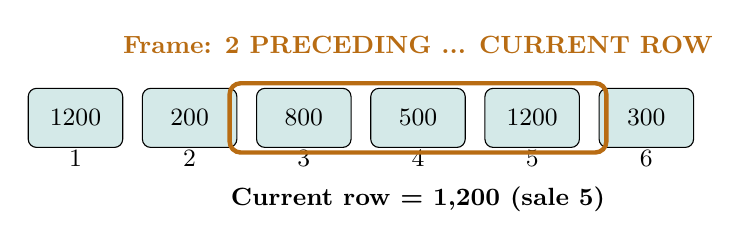
\begin{tikzpicture}[x=1.45cm,y=.8cm,every node/.style={font=\small}]
\foreach \i/\val in {0/1200,1/200,2/800,3/500,4/1200,5/300}{
\node[draw,rounded corners=3pt,minimum width=1.2cm,minimum height=.75cm,fill={TealMain!17}] at (\i,0) {\val};
\node at (\i,-.65) {\pgfmathparse{int(\i+1)}\pgfmathresult};
}
\draw[ultra thick,OrangeMain,rounded corners=4pt] (1.35,-.55) rectangle (4.65,.55);
\node[OrangeMain] at (3,1.15) {\bfseries Frame: 2 PRECEDING ... CURRENT ROW};
\node at (3,-1.3) {\textbf{Current row = 1,200 (sale 5)}};
\end{tikzpicture}
\end{center}
\vspace{.35em}
\begin{itemize}
\item \textbf{Partition} là nhóm rows liên quan.
\item \textbf{Order} tạo vị trí logic trong nhóm.
\item \textbf{Frame} là đoạn con trong partition mà hàm đang xét.
\item Sale 5: frame = 800, 500, 1,200 $\Rightarrow$ AVG = \textbf{833.33}.
\end{itemize}

\end{frame}

% ---- Slide 34 ----
\begin{frame}[fragile]{ROWS và RANGE: cùng ngày, kết quả khác nhau}

\small
\begin{center}
\renewcommand{\arraystretch}{1.18}
\begin{tabular}{rlrrr}
\toprule
sale & date & amount & Default RANGE & Explicit ROWS \\
\midrule
1 & 2026-01-03 & 1,200 & 1,400 & 1,200 \\
2 & 2026-01-03 & 200 & 1,400 & 1,400 \\
3 & 2026-01-12 & 800 & 2,200 & 2,200 \\
\bottomrule
\end{tabular}
\end{center}
\vspace{0.55em}
\begin{columns}[T,onlytextwidth]
\column{.51\textwidth}
\begin{block}{RANGE ... CURRENT ROW}
Khi order theo \code{sale_date}, các giao dịch cùng ngày là peers; frame có thể bao gồm \textbf{cả nhóm peers}.
\end{block}
\column{.49\textwidth}
\begin{block}{ROWS ... CURRENT ROW}
Khi order theo \code{sale_date, sale_id}, running total đi \textbf{từng dòng} một.
\end{block}
\end{columns}

\end{frame}

% ---- Slide 35 ----
\begin{frame}[fragile]{Cú pháp frame: những biên quan trọng}

\begin{center}
\renewcommand{\arraystretch}{1.18}
\begin{tabular}{ll}
\toprule
Boundary & Ý nghĩa \\
\midrule
\code{UNBOUNDED PRECEDING} & Đầu partition \\
\code{N PRECEDING} & N vị trí / giá trị trước \\
\code{CURRENT ROW} & Dòng hiện tại (RANGE gồm peers) \\
\code{N FOLLOWING} & N vị trí / giá trị sau \\
\code{UNBOUNDED FOLLOWING} & Cuối partition \\
\bottomrule
\end{tabular}
\end{center}
\vspace{0.25em}
\begin{beamercolorbox}[wd=\linewidth,sep=1.1ex,rounded=true]{insight}
Với ordered aggregate nhưng \textbf{không khai báo frame}, mặc định MySQL sử dụng \code{RANGE BETWEEN UNBOUNDED PRECEDING AND CURRENT ROW}.
\end{beamercolorbox}
\end{frame}

% ---- Slide 36 ----
\begin{frame}[fragile]{Các frame thường dùng}
\begin{lstlisting}[basicstyle=\ttfamily\fontsize{9.2}{10.399999999999999}\selectfont]
-- Running total by record
ROWS BETWEEN UNBOUNDED PRECEDING AND CURRENT ROW

-- Moving average of at most 3 records
ROWS BETWEEN 2 PRECEDING AND CURRENT ROW

-- Centered 3-record window
ROWS BETWEEN 1 PRECEDING AND 1 FOLLOWING

-- First or last value of whole partition
ROWS BETWEEN UNBOUNDED PRECEDING AND UNBOUNDED FOLLOWING
\end{lstlisting}\vspace{.3em}\small\textbf{Lưu ý:} không phải mọi window function đều phụ thuộc frame; ví dụ ranking dùng ordering/partition, không tính trên moving frame.
\end{frame}

% ---- Slide 37 ----
\begin{frame}[fragile]{Named windows: dùng lại cùng một định nghĩa}
\begin{columns}[T,onlytextwidth]
\column{0.63\textwidth}
\begin{lstlisting}[basicstyle=\ttfamily\fontsize{7.9}{9.1}\selectfont]
SELECT sale_id, sales_rep,
       sale_date, amount,
  ROW_NUMBER() OVER w AS sale_no,
  LAG(amount) OVER w AS prev_amount
FROM sales
WINDOW w AS (
  PARTITION BY sales_rep
  ORDER BY sale_date, sale_id
)
ORDER BY sales_rep, sale_date, sale_id;
\end{lstlisting}
\column{0.37\textwidth}

\textbf{Ưu điểm}\par
\begin{itemize}
\item Tránh lặp định nghĩa window.
\item Hạn chế lỗi thứ tự không thống nhất.
\item Dễ đọc và bảo trì.
\item Có thể định nghĩa nhiều windows với các frames khác nhau.
\end{itemize}
\small \code{WINDOW} đứng trước final \code{ORDER BY}.

\end{columns}
\end{frame}

% ---- Slide 38 ----
\begin{frame}[fragile]{Named windows: cùng order, khác frame}
\begin{lstlisting}[basicstyle=\ttfamily\fontsize{8.2}{9.399999999999999}\selectfont]
SELECT sale_id, sales_rep, amount,
  SUM(amount) OVER w_running AS cumulative,
  AVG(amount) OVER w_last3 AS moving_avg
FROM sales
WINDOW
 w_running AS (
   PARTITION BY sales_rep ORDER BY sale_date, sale_id
   ROWS BETWEEN UNBOUNDED PRECEDING AND CURRENT ROW
 ),
 w_last3 AS (
   PARTITION BY sales_rep ORDER BY sale_date, sale_id
   ROWS BETWEEN 2 PRECEDING AND CURRENT ROW
 );
\end{lstlisting}\begin{beamercolorbox}[wd=\linewidth,sep=1.1ex,rounded=true]{insight}
Ở sale 5 của An: \code{cumulative = 3900}; \code{moving_avg = 833.33}.
\end{beamercolorbox}
\end{frame}

% ---- Slide 39 ----
\begin{frame}[fragile]{Aggregate trước, window sau: đúng đơn vị phân tích}

\begin{center}
\begin{tikzpicture}[node distance=.7cm,every node/.style={font=\small}]
\node[draw,rounded corners,fill=BlueMain!9,minimum width=2.45cm,minimum height=.85cm] (a) {Từng giao dịch};
\node[draw,rounded corners,fill=TealMain!8,minimum width=3.0cm,minimum height=.85cm,right=of a] (b) {GROUP BY rep, month};
\node[draw,rounded corners,fill=OrangeMain!11,minimum width=3.3cm,minimum height=.85cm,right=of b] (c) {LAG theo từng rep};
\draw[-{Stealth},thick] (a)--(b);\draw[-{Stealth},thick](b)--(c);
\end{tikzpicture}
\end{center}
\begin{lstlisting}[basicstyle=\ttfamily\fontsize{8.0}{9.2}\selectfont]
WITH monthly AS (
 SELECT sales_rep, DATE_FORMAT(sale_date, '%Y-%m-01') AS mon,
        SUM(amount) AS monthly_total
 FROM sales
 GROUP BY sales_rep, DATE_FORMAT(sale_date, '%Y-%m-01')
)
SELECT sales_rep, mon, monthly_total,
       LAG(monthly_total) OVER (
         PARTITION BY sales_rep ORDER BY mon
       ) AS prev_month
FROM monthly;
\end{lstlisting}
\end{frame}

% ---- Slide 40 ----
\begin{frame}[fragile]{Monthly analytics: ví dụ của An}

\begin{center}
\renewcommand{\arraystretch}{1.18}
\begin{tabular}{lrrr}
\toprule
Month & Monthly revenue & Previous month & Change \\
\midrule
2026-01 & 2,200 & NULL & NULL \\
2026-02 & 1,700 & 2,200 & -500 \\
2026-03 & 300 & 1,700 & -1,400 \\
\bottomrule
\end{tabular}
\end{center}
\vspace{0.9em}
\begin{itemize}
\item Running monthly revenue: \textbf{2,200 $\to$ 3,900 $\to$ 4,200}.
\item Cần phân tích theo tháng: \textbf{GROUP BY month trước}, rồi mới dùng \code{LAG}.
\item Nếu một tháng không có giao dịch, \code{LAG} lấy row tháng có dữ liệu trước đó; muốn tháng liên tục phải tạo calendar/time spine.
\end{itemize}

\end{frame}

% ---- Slide 41 ----
\begin{frame}[fragile]{Giới hạn của MySQL Window Functions}

\begin{columns}[T,onlytextwidth]
\column{.49\textwidth}
\begin{block}{Dùng trực tiếp}
\begin{itemize}
\item \code{SELECT} list
\item \code{ORDER BY}
\end{itemize}
\end{block}
\begin{alertblock}{Không dùng trực tiếp}
\begin{itemize}
\item \code{WHERE}, \code{HAVING}
\item \code{GROUP BY}, \code{JOIN ... ON}
\item \code{UPDATE ... SET} cùng query block
\end{itemize}
\end{alertblock}
\column{.51\textwidth}
\textbf{Một số constructs không hỗ trợ:}
\begin{itemize}
\item Nested window functions.
\item \code{DISTINCT} trong aggregate window.
\item \code{GROUPS} frame, \code{EXCLUDE}.
\item \code{IGNORE NULLS}.
\item \code{NTH_VALUE ... FROM LAST}.
\end{itemize}
\small\textit{Sử dụng CTE/derived tables khi cần thêm lớp tính toán.}
\end{columns}

\end{frame}

% ---- Slide 42 ----
\begin{frame}[fragile]{Những lỗi cần nhớ khi thực hành}

\small
\begin{center}
\renewcommand{\arraystretch}{1.18}
\begin{tabular}{ll}
\toprule
Lỗi & Cách khắc phục \\
\midrule
Dùng GROUP BY khi cần từng sale & Dùng aggregate \code{OVER(PARTITION BY ...)} \\
\code{ROW_NUMBER} thiếu tie-break & Thêm primary key vào window ordering \\
\code{RANK} cho exactly N rows & Dùng \code{ROW_NUMBER} \\
Running SUM mặc định dùng RANGE & Viết \code{ROWS} explicit \\
\code{LAST_VALUE} sai giá trị cuối & Khai báo full-partition frame \\
Filter rank ngay trong WHERE & Tách CTE và outer WHERE \\
Nhầm order trong OVER với output & Viết final ORDER BY \\
\bottomrule
\end{tabular}
\end{center}
\end{frame}

% ---- Slide 43 ----
\begin{frame}[fragile]{WHERE lọc trước window: khác biệt nghiệp vụ}
\begin{columns}[T,onlytextwidth]
\column{0.60\textwidth}
\begin{lstlisting}[basicstyle=\ttfamily\fontsize{8.1}{9.299999999999999}\selectfont]
-- Revenue within Feb-Mar only
SELECT region, sale_id, amount,
 SUM(amount) OVER (
   PARTITION BY region
 ) AS total_after_filter
FROM sales
WHERE sale_date >= '2026-02-01';
\end{lstlisting}
\column{0.40\textwidth}

\textbf{Kết quả}\par
\begin{itemize}
\item North: \textbf{3,050} (Feb--Mar).
\item South: \textbf{2,750} (Feb--Mar).
\end{itemize}
\vspace{0.4em}
Nếu muốn \textbf{tổng cả lịch sử} nhưng chỉ hiển thị sale từ tháng 2: tính window trong CTE trước, rồi filter ngày ở outer query.

\end{columns}
\end{frame}

% ---- Slide 44 ----
\begin{frame}[fragile]{Performance: kiểm tra thay vì suy đoán}
\begin{columns}[T,onlytextwidth]
\column{0.61\textwidth}
\begin{lstlisting}[basicstyle=\ttfamily\fontsize{8.1}{9.299999999999999}\selectfont]
EXPLAIN
SELECT sale_id, sales_rep,
 SUM(amount) OVER (
   PARTITION BY sales_rep
   ORDER BY sale_date, sale_id
   ROWS BETWEEN UNBOUNDED PRECEDING
            AND CURRENT ROW
 ) AS running_revenue
FROM sales;
\end{lstlisting}
\column{0.39\textwidth}

\textbf{Chi phí phụ thuộc:}
\begin{itemize}
\item Số rows và số partitions.
\item Sort, memory và temporary data.
\item Điều kiện lọc, indexes và query plan.
\item Server version và configuration.
\end{itemize}
\small Index khớp với partition/order có thể hữu ích, \textbf{không đảm bảo} loại bỏ mọi sort.

\end{columns}
\end{frame}

% ---- Slide 45 ----
\begin{frame}[fragile]{Mở rộng classicmodels: customer payments}
\begin{lstlisting}[basicstyle=\ttfamily\fontsize{8.5}{9.7}\selectfont]
SELECT customerNumber, paymentDate, checkNumber, amount,
 SUM(amount) OVER (
   PARTITION BY customerNumber
   ORDER BY paymentDate, checkNumber
   ROWS BETWEEN UNBOUNDED PRECEDING AND CURRENT ROW
 ) AS running_paid_amount,
 LAG(amount) OVER (
   PARTITION BY customerNumber
   ORDER BY paymentDate, checkNumber
 ) AS previous_payment
FROM classicmodels.payments
ORDER BY customerNumber, paymentDate, checkNumber;
\end{lstlisting}\small\textit{Chỉ chạy nếu đã cài \code{classicmodels}. Sử dụng \code{checkNumber} để phá hòa khi một customer có nhiều payment cùng ngày.}
\end{frame}

% ---- Slide 46 ----
\begin{frame}[fragile]{Thực hành A: window aggregate và frame}

\begin{enumerate}
\setlength{\itemsep}{.72em}
\item Hiển thị \code{sale_id, region, sales_rep, amount} kèm \textbf{company total}, \textbf{region total} và \textbf{percentage in region}.
\item Với mỗi nhân viên, tính \textbf{running revenue} theo \code{sale_date, sale_id}.
\item Với mỗi nhân viên, tính \textbf{moving average} của tối đa 3 giao dịch gần nhất.
\item So sánh hai running totals cho An: dùng default \code{RANGE} và explicit \code{ROWS}.
\item Lọc ra sales có \code{amount} lớn hơn average amount của \code{region} tương ứng.
\end{enumerate}

\end{frame}

% ---- Slide 47 ----
\begin{frame}[fragile]{Thực hành B: ranking và value functions}

\begin{enumerate}
\setlength{\itemsep}{.72em}
\item Viết 3 truy vấn lấy top 2 sale theo mỗi region: \textbf{exactly 2 rows}, \textbf{giữ ties}, \textbf{2 amount levels}.
\item Ghi thứ tự \code{ROW_NUMBER}, \code{RANK}, \code{DENSE_RANK} cho dãy: \textbf{100, 100, 80, 50}.
\item Với mỗi sale, tính amount trước, amount sau và chênh lệch amount trước.
\item Hiển thị first sale, last sale và second sale amount theo nhân viên.
\item Chia sales của từng region thành 4 nhóm bằng \code{NTILE(4)}; giải thích ties.
\end{enumerate}

\end{frame}

% ---- Slide 48 ----
\begin{frame}[fragile]{Mini-project 1: Sales dashboard}

\textbf{Viết một query trên bảng \code{sales} để trả về:}
\begin{enumerate}
\setlength{\itemsep}{.6em}
\item \code{sale_id, region, sales_rep, sale_date, amount}.
\item Tổng doanh thu \textbf{toàn công ty} và \textbf{theo region}.
\item Mức doanh thu \textbf{trung bình của region}.
\item Tỷ trọng \textbf{\% của sale} trong region.
\item \code{RANK()} giữ ties theo amount và \code{ROW_NUMBER()} deterministic.
\item Sắp đầu ra theo region, rank và sale ID.
\end{enumerate}
\vspace{0.3em}
\begin{beamercolorbox}[wd=\linewidth,sep=1.1ex,rounded=true]{insight}
\textbf{Kiểm thử:} company total = 14,200; North = 7,350; South = 6,850.
\end{beamercolorbox}
\end{frame}

% ---- Slide 49 ----
\begin{frame}[fragile]{Mini-project 2: Rep performance analytics}

\textbf{Đầu ra cho từng nhân viên, theo trình tự thời gian:}
\begin{itemize}
\setlength{\itemsep}{.5em}
\item Số thứ tự giao dịch: \code{ROW_NUMBER()}.
\item Giao dịch trước và sau: \code{LAG()}, \code{LEAD()}.
\item Thay đổi so với giao dịch trước.
\item Tổng lũy kế: \code{SUM() OVER(... ROWS ...)}.
\item Moving average của 3 giao dịch.
\item Amount của giao dịch đầu và cuối toàn partition.
\end{itemize}
\vspace{0.3em}
\textbf{Gợi ý:} Định nghĩa các named windows \code{w_order}, \code{w_running}, \code{w_last3}, \code{w_full}.

\end{frame}

% ---- Slide 50 ----
\begin{frame}[fragile]{Mini-project 3: Monthly sales analytics}

\begin{enumerate}
\setlength{\itemsep}{.7em}
\item Tạo CTE doanh thu theo \code{region} và \code{month}.
\item Tính doanh thu tháng trước bằng \code{LAG}.
\item Tính \textbf{month-over-month change} và running monthly revenue.
\item Chỉ lấy các tháng có doanh thu tăng so với tháng trước (outer query).
\item Thảo luận tháng không có doanh thu: \code{LAG} đang so sánh với tháng lịch liền trước hay row trước đó?
\end{enumerate}
\vspace{0.45em}
\begin{beamercolorbox}[wd=\linewidth,sep=1.1ex,rounded=true]{insight}
\textbf{Mục tiêu cốt lõi:} Chọn đúng \emph{grain} (đơn vị phân tích), sau đó mới chọn window function.
\end{beamercolorbox}
\end{frame}

% ---- Slide 51 ----
\begin{frame}[fragile]{Câu hỏi nhanh kiểm tra kiến thức}

\begin{enumerate}
\setlength{\itemsep}{.8em}
\item \code{SUM(amount) OVER(PARTITION BY region)} có làm giảm số rows không?
\item Muốn lấy đúng 3 dòng theo mỗi region dùng \code{RANK} hay \code{ROW_NUMBER}?
\item Để running total đi từng giao dịch khi có nhiều giao dịch cùng ngày, nên dùng \code{ROWS} hay \code{RANGE}?
\item Vì sao \code{LAST_VALUE} cần full frame để lấy giao dịch cuối cùng?
\item Muốn lọc \code{row_num <= 3}, vì sao cần thêm query layer?
\end{enumerate}

\end{frame}

% ---- Slide 52 ----
\begin{frame}[fragile]{Đáp án kiểm tra nhanh}

\begin{enumerate}
\setlength{\itemsep}{.85em}
\item \textbf{Không.} Window aggregate giữ các detail rows.
\item \textbf{ROW\_NUMBER.} Có tie-breaker để chọn tối đa 3 dòng.
\item \textbf{ROWS} với thứ tự xác định, ví dụ \code{sale_date, sale_id}.
\item Default frame của ordered window thường chỉ đến current row, chưa đến cuối partition.
\item Window calculation không dùng trực tiếp trong \code{WHERE} cùng query block; tính trong CTE rồi lọc ở query ngoài.
\end{enumerate}

\end{frame}

% ---- Slide 53 ----
\begin{frame}[fragile]{Tổng kết: chọn window function theo nhu cầu}

\small
\begin{center}
\renewcommand{\arraystretch}{1.18}
\begin{tabular}{ll}
\toprule
Câu hỏi phân tích & Công cụ chính \\
\midrule
Tổng/avg theo nhóm, giữ detail & \code{SUM/AVG(...) OVER(PARTITION BY ...)} \\
Doanh thu tích lũy / rolling avg & Aggregate window + explicit \code{ROWS} \\
Đánh số, ranking, top-N & \code{ROW_NUMBER/RANK/DENSE_RANK} \\
So sánh các thời điểm liên tiếp & \code{LAG/LEAD} \\
Giá trị đầu/cuối/thứ N & \code{FIRST/LAST/NTH_VALUE} \\
Phân vị, vị trí trong phân phối & \code{NTILE/PERCENT_RANK/CUME_DIST} \\
Loại bỏ theo kết quả window & \code{CTE} / derived table \\
\bottomrule
\end{tabular}
\end{center}
\end{frame}

% ---- Slide 54 ----
\begin{frame}[fragile]{Tài liệu và hướng dẫn thực hành}

\begin{itemize}
\setlength{\itemsep}{.82em}
\item \textbf{Bài giảng gốc:} \href{https://vudmvn.github.io/dbms-course/lectures/MySQL/querying-data/window-functions/window-functions/}{DBMS Course -- MySQL Window Functions}.
\item \textbf{MySQL Reference Manual:} \href{https://dev.mysql.com/doc/refman/8.4/en/window-functions.html}{Window Function Descriptions}.
\item \textbf{Cú pháp và frame:} \href{https://dev.mysql.com/doc/refman/8.4/en/window-functions-frames.html}{Window Function Frame Specification}.
\item \textbf{Chuẩn bị:} MySQL 8.0+, schema \code{window_function_lab}; có thể mở rộng với \code{classicmodels}.
\item \textbf{File đi kèm:} \code{window_functions_lab.sql} cung cấp dữ liệu mẫu và kiểm thử.
\end{itemize}
\vspace{1em}
\begin{center}{\Large\bfseries Cảm ơn!}\end{center}

\end{frame}
\end{document}
